\documentclass{article}
\usepackage{color}
\usepackage{here}
  \usepackage{url}
\usepackage[dvipdfmx]{graphicx}
\usepackage[dvipdfmx]{hyperref}
\title{Compare mesher}
\begin{document}


\maketitle 
\section*{Implicit surface meshing}
In order to obtain a deformed surface, we need to compute a triangle mesh implementation of the implicit surface computed with surface reconstruction algorithm.
\subsection*{Marching Cubes}
Marching Cubes is an algorithm for rendering isosurfaces from volumetric data. The basic idea is to consider a bounding box for the object to be meshed and subdivide it regularly into smaller cells Then the function $f$ is sampled at the eight corners of each cell. If one or more values is less than the user-specified isovalue, and one or more have values is greater than this isovalue, the cell must intersect the isosurface. By determining the edges in the cell that are intersected by the isosurface, and connecting them we can form a linear approximation of the surface in each cell. By connecting the patches from all cells, we get a linear approximation of the isosurface. 
\subsection*{Delaunay based implicit surface meshing}
Since we know that all the points from the deformed point- cloud belong to the surface of the deformed object (or at least are close to it), Marching Cubes based algorithm do not look like the most effective approach. Instead one could compute a Delaunay tetrahedralization of the deformed point-cloud and peel off outside tetrahedra using the fitted function (either from the HRBF or Poisson surface reconstruction approach). One practical implementation is the implicit surface mesh generator implemented by CGAL which is an implementation of the algorithm of Boissonat and Oudot \cite{cgalDelaunay1}.  Our Delaunay judges whether or not the center of gravity of this tetrahedron is on the surface of the object and efficiency is good more than CGAL Delaunay which calculates the whole object.

\section*{Experiment}

This experiment compares the running time of different meshing algorithms, combined with an implicit surface reconstruction algorithm, for the purpose of reconstructing a surface from a set of points sampled on a surface.
Given an implicitly defined unit sphere, we compute a triangle mesh approximation using the Marching Cubes algorithm. We use different grid resolutions for the Marching Cubes algorithm, in order to create triangle meshes with different number of vertices and triangles. These triangle meshes will be used as the input data for comparing the different meshing algorithms.
\\
Three different meshing algorithms are compared:\\
- The Marching Cubes algorithm \cite{marching}\\
- A meshing algorithm based on a Delaunay triangulation of the input point-cloud \cite{ourDelaunay1}\\
- The implicit surface meshing algorithm of CGAL \cite{cgalDelaunay1}, \cite{cgalDelaunay2}\\, \cite{cgalDelaunay3}

These meshing algorithms are applied to a function obtained either by the Poisson surface reconstruction algorithm or by fitting a compactly supported Hermite Radial Basis Function (HRBF).
Overall, we are expecting the Delaunay based surface mesher to be the most efficient, because we already have a sampling of the surface to start with. By comparison the Marching Cubes algorithm needs to always sample the reconstructed function on a regular grid, which can be expensive if the grid has a high resolution.
The CGAL implicit surface mesher is using a more sophisticated sampling algorithm to probe the surface, and is thus relatively expensive. When using the CGAL surface mesher in the experiments below, we use as an input sampling of the surface the points from the input point-cloud.

Tables 1 to 8 below show the running time obtained by the different meshing algorithms for reconstructing a unit sphere from point-clouds with different sizes.\\
\\
\noindent
\begin{table}
 \caption{Closed-form approximation HRBF reconstruction and meshing from a sphere with 480 vertices and 956 faces. The input mesh was obtained with the Marching Cubes algorithm using a grid resolution of $16^3$.}
  \begin{tabular}{|l|c|c|c|} \hline
    Mesh algoritms & Marching Cubes & Our Delaunay & CGAL Delaunay \\  \hline
    Time[ms] & 40 & 30 & 4936\\ \hline
    Number of vertices and faces after mesh & 552, 1096 & 480, 954 &2102, 4196 \\ \hline
  \end{tabular}
\end{table}

\begin{table}
 \caption{Poisson reconstruction and meshing from a sphere with 480 vertices and 956 faces. The input mesh was obtained with the Marching Cubes algorithm using a grid resolution of $16^3$}
\noindent
  \begin{tabular}{|l|c|c|c|} \hline
    Mesh algoritms & Marching Cubes & Our Delaunay & CGAL Delaunay \\  \hline
    Time[ms] & 7 & 25 & 1034\\ \hline
    Number of vertices and faces after mesh & 480, 956 & 480, 930 &1719, 3434 \\ \hline
  \end{tabular}
\end{table}

\begin{table}
 \caption{Closed-form approximation HRBF reconstruction and meshing from a sphere with 1992 vertices and 3980 faces. The input mesh was obtained with the Marching Cubes algorithm using a grid resolution of $32^3$.}
\noindent

  \begin{tabular}{|l|c|c|c|} \hline
    Mesh algoritms & Marching Cubes & Our Delaunay & CGAL Delaunay \\  \hline
    Time[ms] & 646 & 80 & 21669\\ \hline
    Number of vertices and faces after mesh & 2736, 5464 & 1992, 3970 &4769, 9530 \\ \hline
  \end{tabular}
\end{table}

\begin{table}
 \caption{Poisson reconstruction and meshing from a sphere with 1992 vertices and 3980 faces. The input mesh was obtained with the Marching Cubes algorithm using a grid resolution of $32^3$}
\noindent 
  \begin{tabular}{|l|c|c|c|} \hline
    Mesh algoritms & Marching Cubes & Our Delaunay & CGAL Delaunay \\  \hline
    Time[ms] & 40 & 87 & 2118\\ \hline
    Number of vertices and faces after mesh & 2004, 4004 & 1992, 3628 &3887, 7766 \\ \hline
  \end{tabular}
\end{table}

\begin{table}
 \caption{Closed-form approximation HRBF reconstruction and meshing from a sphere with 8376 vertices and 16748 faces. The input mesh was obtained with the Marching Cubes algorithm using a grid resolution of $64^3$.}
\noindent
  \begin{tabular}{|l|c|c|c|} \hline
    Mesh algoritms & Marching Cubes & Our Delaunay & CGAL Delaunay \\  \hline
    Time[ms] & 24407 & 360 & 622310\\ \hline
    Number of vertices and faces after mesh & 13944, 27880 & 8376, 16754 &21143, 42274 \\ \hline
  \end{tabular}
\end{table}

\begin{table}
 \caption{Poisson reconstruction and meshing from a sphere with 8376 vertices and 16748 faces. The input mesh was obtained with the Marching Cubes algorithm using a grid resolution of $64^3$.}
\noindent
Poisson\\
  \begin{tabular}{|l|c|c|c|} \hline
    Mesh algoritms & Marching Cubes & Our Delaunay & CGAL Delaunay \\  \hline
    Time[ms] & 221 & 256 & 16276\\ \hline
    Number of vertices and faces after mesh & 8378, 16752 & 8376, 14665 &20876, 41748 \\ \hline
  \end{tabular}
\end{table}

\begin{table}
 \caption{Poisson reconstruction and meshing from a sphere with 33696 vertices and 67388 faces. The input mesh was obtained with the Marching Cubes algorithm using a grid resolution of $128^3$.}
  \begin{tabular}{|l|c|c|c|} \hline
    Mesh algoritms & Marching Cubes & Our Delaunay & CGAL Delaunay \\  \hline
    Time[ms] & 1332 & 1133 & 73303\\ \hline
    Number of vertices and faces after mesh & 33696, 67388 & 33696, 55877 &76641, 153278 \\ \hline
  \end{tabular}
 \end{table} 
 



\begin{table}
 \caption{Poisson reconstruction and meshing from a sphere with 136224 vertices and 272444 faces. The input mesh was obtained with the Marching Cubes algorithm using a grid resolution of $256^3$.}
  \begin{tabular}{|l|c|c|c|} \hline
    Mesh algoritms & Marching Cubes & Our Delaunay & CGAL Delaunay \\  \hline
    Time[ms] & 9763 & 3695 & 408205\\ \hline
    Number of vertices and faces after mesh & 136222, 272440& 136224, 185169 &343567, 686970 \\ \hline
  \end{tabular}

\end{table}

We remark in the previous tables that the number of vertices (and faces) is higher than the expected number of vertices (for a given the grid resolution), when the Marching Cubes algorithm is used to mesh the function obtained from HRBF fitting.
The problem comes from the fact that compactly supported splines are used, and they create additional zero iso-surfaces away from the object surface. It is not difficult to modify the Marching Cubes algorithm in order to ignore these extra surfaces. However, this does not impact much the running time of the Marching Cubes, since the bottleneck is in sampling the function on the regular grid. Therefore, we did not bother writing additional code to ignore these extra surfaces.

\begin{figure}[h]
\begin{center}
\caption{Marching Cubes, Our Delaunay and CGAL Delaunay time}
 \label{fig:threegraph}
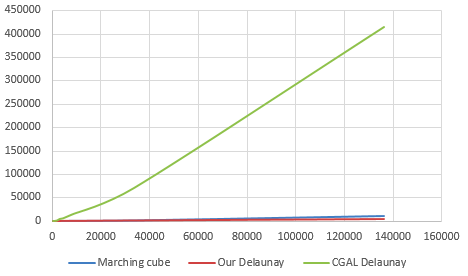
\includegraphics[width=10cm]{compare_mesher_graph.png}

\end{center}
\end{figure}

\begin{figure}[h]
\begin{center}
\caption{Our Delaunay and CGAL Delaunay time}
 \label{fig:twograph}
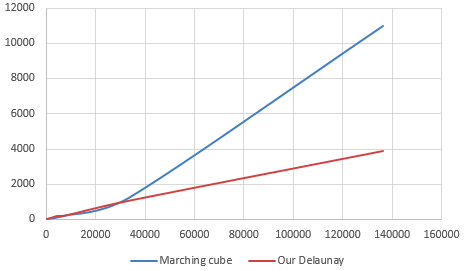
\includegraphics[width=10cm]{marching_and_delaunay_timegraph.png}

\end{center}
\end{figure}
Figure \ref{fig:threegraph} and Figure \ref{fig:twograph} show the running time in milliseconds for the three different meshing algorithms, when the Poisson surface reconstruction method is used. The running times are given for input of different sizes. The horizontal axis corresponds to the number of points in the input point-cloud.\\
Time complexity for evaluating at one point the function obtained from the Poisson surface reconstruction is  $O(v^{\frac{1}{3} }) $. where v is the number of points in the input point-cloud. 
Marching Cubes time complexity is $O(n^3 v^{\frac{1}{3} })$. n is grid resolution. When the number of vertices is small, it is faster than other meshers. The more vertices the more it will take more time.\\
The worst time complexity of the Delaunay based mesher is $O(v^2\times v^{ \frac{1}{3} })$. However, A paper of Attali and Boissonnat \cite{ourDelaunay2} suggests that the time complexity in Delaunay triangulation is linear when points are sampled in 3D on the surface of the object. Thus, we should expect in practice a complexity of $O(v\times v^{ \frac{1}{3} })$. When the number of vertices is small, it is slower than the Marching Cubes, but as the number of points increases, it becomes the fastest meshing algorithm.\\
CGAL Delaunay is difficult to evaluate its time complexity. CGAL Delaunay adding samples based on some condition.  The increase in time when the number of vertices is increased is large, this was the slowest algorithm.

\section*{Conclusion}
These experiments seem to indicate that the Delaunay-based meshing algorithm is preferable for our use case.
In addition to being slower for our particular case, the Marching Cubes algorithm has the following disadvantages over the Delaunay based implicit surface mesher:\\
- It generates poor shaped triangle,\\
- It is difficult to estimate the grid resolution to use in order to maintain approximately the number of vertices on the surface.


 \begin{thebibliography}{9}
 \bibitem{marching}
 William E. Lorensen and Harvey E. Cline. 1987. Marching Cubes: A high resolution 3D surface construction algorithm. SIGGRAPH Comput. Graph. 21, 4 (August 1987), 163-169.
 \bibitem{ourDelaunay1}
 Pierre-Alain Fayolle and Alexander Pasko. 2012. Optimized surface discretization of functionally defined multi-material objects. Adv. Eng. Softw. 45, 1 (March 2012), 301-312.
\bibitem{cgalDelaunay1}
Jean-Daniel Boissonnat and Steve Oudot. Provably good sampling and meshing of surfaces. Graphical Models, 67:405-451, 2005.
\bibitem{cgalDelaunay2}
Laurent Rineau and Mariette Yvinec. A generic software design for Delaunay refinement meshing. Comput. Geom. Theory Appl., 38:100-110, 2007.
 \bibitem{ourDelaunay2}
 Dominique Attali and 2004. Jean-Daniel BoissonnatA linear bound on the Complexity of the Delaunay Triangulation of Points on Polyhedral Surfaces
\bibitem{cgalDelaunay3}
CGAL 4.9.1 - 3D Surface Mesh Generation \\
\url{http://doc.cgal.org/latest/Surface_mesher/group__PkgSurfaceMesher3FunctionsMakeMesh.html}


\end{thebibliography}


\end{document}